\documentclass{article}
\usepackage{graphicx}
\usepackage[utf8]{inputenc}
\usepackage{amsmath}
\usepackage{amssymb}
\usepackage{graphicx}
\usepackage{epstopdf}
\usepackage{inputenc}
\usepackage{latexsym}
\usepackage{setspace}
\usepackage{caption}
\usepackage{authblk}
\usepackage{float}
\setlength\parindent{24pt}
\usepackage[export]{adjustbox}
\usepackage{wrapfig}


\begin{document}

\title{Lasers and Laser Mode Structures}
\author{Loïc James McKeever}
\affil{Mackenzie Levangie}

\maketitle

\section{Introduction}

The objective of this experiment is to observe different types of laser modes and quantify our observations.  Laser modes are due to the boundary conditions imposed by the length of the laser's cavity(distance between the two mirrors) and the radius of curvature of those mirrors.  These parameters create a shift in the wavelength of a portion of a beam and then due to destructive interference a variety of patterns are produced.  In this experiment we are using a laser with an external cavity that can be adjusted.  An interferometer and a spectrum analyzer will be used to determine the shift in frequency for the different modes observed. For the first non-single mode we found a shift of $0.4207 \pm 0.018 GHz$ in the frequency domain.  For the second non-single mode we found shifts of $0.418 \pm 0.018 GHz$ and $0.176 \pm 0.018 GHz$.


\section{Materials and Methods}

In this lab we used an external cavity HeNe laser(model number 05-LHB-570) powered by a Melles Griot power supply(model number 05-LPL-939-065).  The beam was then reflected into a scanning Fabry Perot Interferometer(ThorLabs model number SA200) connected to a Spectrum Analyzer(ThorLabs model number SA201) with an oscilloscope(Tektronix model number TDS 210) used as a display.  See Figures 1, 2 and 3 for detailed set-ups of the external cavity laser, Interferometer/Spectrum Anaylzer/Oscilloscope and the overall experimental set-up.  The power of the laser was measured with an optical power meter(ThorLabs model number PM100).  The data was gathered from the oscilloscope using Tektronix software.  The data was on a time scale but knowing the Free Spectral Range(FSR) for our interferometer(1.5 GHz) and the wavelength of our laser(632.8 nm) we could convert the time scale to either nm scale or GHz scale. 

\begin{figure}[H]
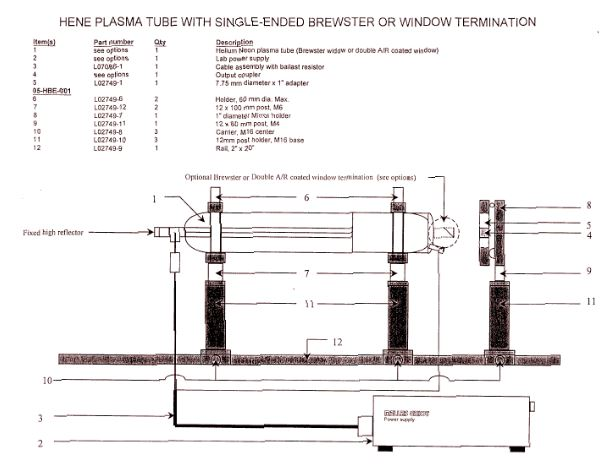
\includegraphics[scale=0.6,center]{Laser.JPG}
\caption{Diagram of external cavity HeNe laser.$^{[1]}$}
\end{figure}

\begin{figure}[H]
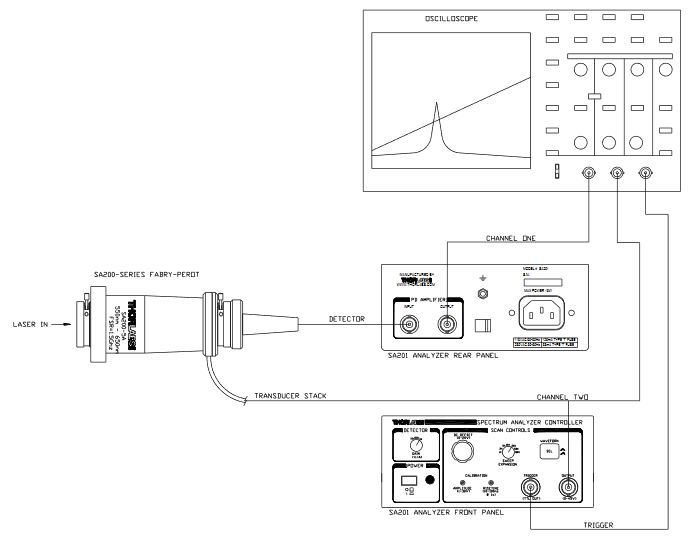
\includegraphics[scale=0.6,center]{Interferometer.JPG}
\caption{Diagram of recommended set-up of the interferometer, spectrum analyzer and oscilloscope.$^{[2]}$}
\end{figure}

\begin{figure}[H]
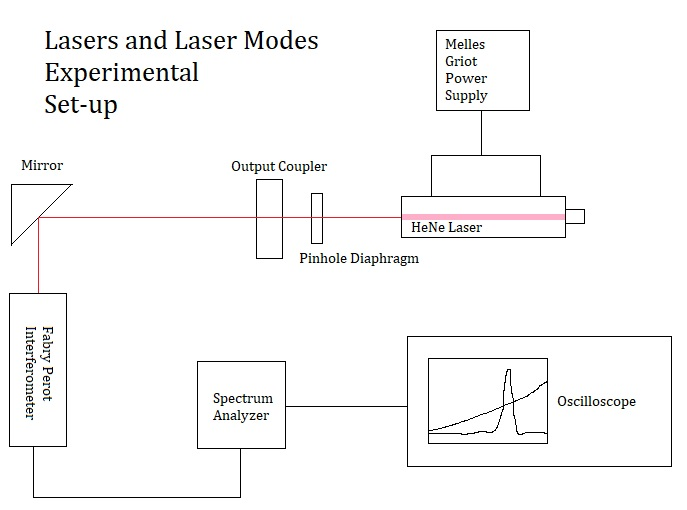
\includegraphics[scale=0.6,center]{LaserSetup.jpg}
\caption{Diagram of the general experimental set-up used in this lab.}
\end{figure}

\newpage 

\section{Results}

\begin{wrapfigure}[10]{R}{0}
  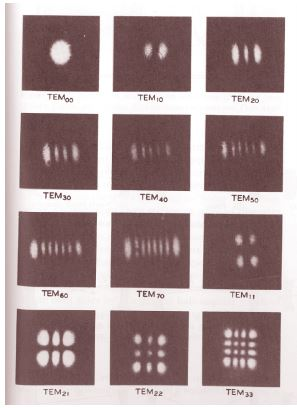
\includegraphics[scale=0.6]{LaserModesChart.JPG}
  \caption{Spatial laser modes and their designations.$^{[3]}$}
\end{wrapfigure}

We started with simply identifying as many modes from Figure 4 as we could by adjusting the cavity length, the angle of the output coupler(the coupler could be tilted downward and to the side) and the size of the pinhole.  We were able to find eight of the twelve shown in Figure 4.  Figures 5 through 7 show our results for 3 separate cavity lengths.  These results aren't quantitative but they do give us an idea about what sort of factors determine what modes are achieved.  
\\
\\
\\
\\
\\
\\
\\
\\
\begin{figure}[H]
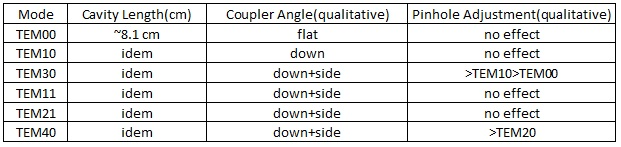
\includegraphics[scale=0.6,center]{Table1.jpg}
\caption{Table of modes achieved with a cavity length of 8.1 cm.}
\end{figure}

\begin{figure}[H]
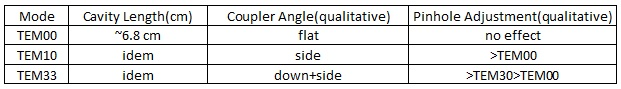
\includegraphics[scale=0.6,center]{Table2.jpg}
\caption{Table of modes achieved with a cavity length of 6.8 cm.}
\end{figure}

\begin{figure}[H]
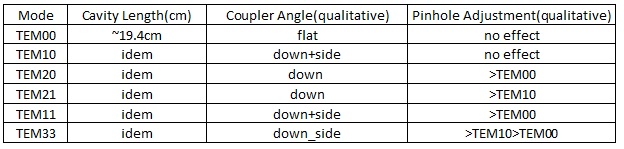
\includegraphics[scale=0.6,center]{Table3.jpg}
\caption{Table of modes achieved with a cavity length of 19.4 cm.}
\end{figure}


\newpage

Then laser's cavity length was then set to $L=36.195 \PM 0.0794 cm$ and we gathered data at three separate modes; TEM00, TEM10 and TEM20.   The power for each of these modes was measured to be $60 \mu W$. $90 \mu W$ and $260 \mu W$ respectively.  Figures 8 through 9 show the Frequency Spectrum of each of these nodes.  The mirrors of the laser have a radius of convergence to be $R=45cm$.  From these values we can determine the changes in frequency we should expect.  The frequency of a particular cavity mode depends on all three mode numbers.  Changing the longitudinal mode number by one changes the frequency by
\begin{equation}
\Delta\nu_{long}=\frac{c}{2L}
\end{equation}
Changing either of the transverse mode
numbers by 1 changes the frequency by
\begin{equation}
\Delta\nu_{tran}=\frac{c}{\pi L}tan^{-1}(\frac{L}{2z_{R}})
\end{equation}
where
\begin{equation}
 z_{R}=\frac{1}{2}\sqrt{L(2R-L)}   
\end{equation}

Here we find $\Delta\nu_{long}=0.414 \pm 0.001 GHz$ and $\Delta\nu_{tran}=0.181 \pm 0.0006 GHz$.



\begin{figure}[H]
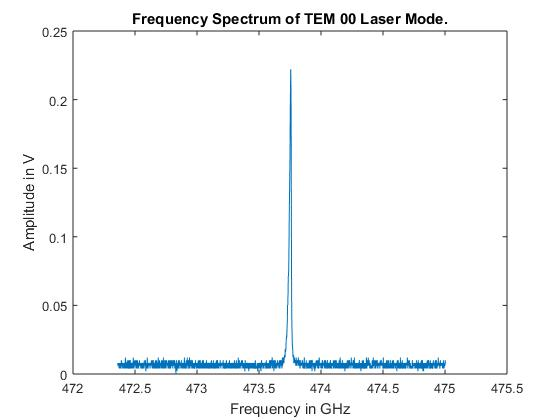
\includegraphics[scale=0.4,center]{TEM00.jpg}
\caption{Frequency Spectrum of a single mode laser.  The peak is located at 632.8 nm and has a FWHM of 0.024 nm which is reasonably precise.  Assuming the distribution is Gaussian that gives us an uncertainty $\sigma=\frac{FWHM}{2.35}=0.009 GHz$.That converts to a FWHM of 0.67 ms on the time scale and 0.0177 GHz on the frequency scale.}
\end{figure}

\begin{figure}[H]
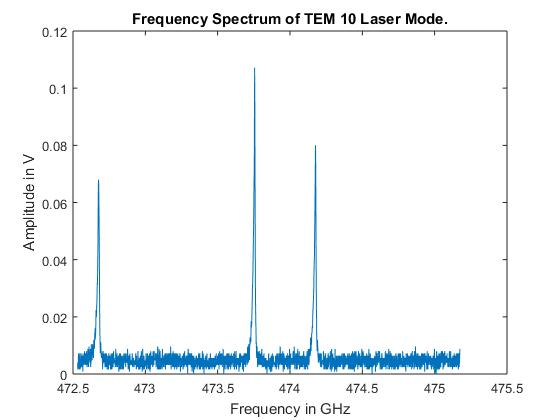
\includegraphics[scale=0.4,center]{TEM10.jpg}
\caption{Frequency Spectrum of the TEM10 mode.  We can see the main peak at 632.8 nm and the second peak due to the frequency being shifted.  The third peak(peak furthest to the left) comes from the signal repeating itself every 0.0568 s due to the FSR of the interferometer.}
\end{figure}

\begin{figure}[H]
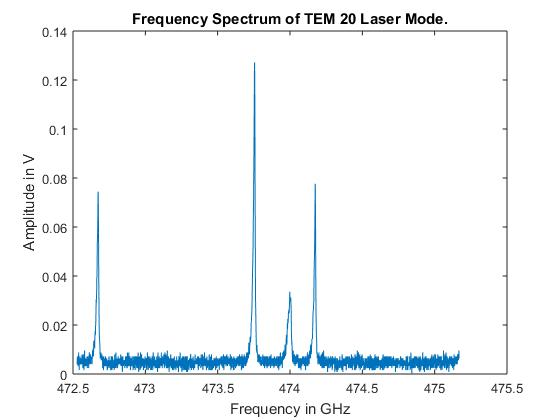
\includegraphics[scale=0.4,center]{TEM20.jpg}
\caption{Frequency Spectrum of the TEM20 mode.  We can see the main peak at 632.8 nm and the two peaks due to the frequency being shifted twice.  The fourth peak(peak furthest to the left) comes from the signal repeating itself every 0.0568 s due to the FSR of the interferometer.}
\end{figure}

In Figure 2 the difference between the two peaks is $0.4207 \pm 0.018 GHz$ in the frequency domain.  In Figure 3 the difference between the main peak and the last peak is $0.418 \pm 0.018 GHz$ and the difference between the last peak and the middle peak is $0.176 \pm 0.018 GHz$.  



\section{Discussion}

For our first mode we expect a shift of $\Delta\nu_{long}=0.414 \pm 0.001 GHz$ from Equation 1 and we found a shift in frequency of $0.4207 \pm 0.018 GHz$ which is consistent.  For our second mode we found frequency shifts of $0.418 \pm 0.018 GHz$ and $0.176 \pm 0.018 GHz$ which is consistent with our expected values of $\Delta\nu_{long}=0.414 \pm 0.001 GHz$ and $\Delta\nu_{tran}=0.181 \pm 0.0006 GHz$.

\section{Conclusion}

In conclusion laser modes depend on three main things; cavity length of the laser, radius of curvature of the mirrors of the laser and the angle of those mirrors.  We were able to observe and quantify the shifts in frequency that generate two different modes; $0.4207 \pm 0.018 GHz$ fro TEM10 and $0.418 \pm 0.018 GHz$ and $0.176 \pm 0.018 GHz$ for TEM20.

\section{References}

[1] Experiment 5: Lasers and Laser Mode Structure Lab Manual, Northeastern University PHYS5318
\\
\\
\noindent [2] SA200-Series Scanning Fabry Perot Interferometer User Manual, ThorLabs
\\
\\
\noindent [3] Hecht, Optics, Addison-Wesley, 2nd Edition

\end{document}
